\begin{remark*}[Standard quantified statement]
For every right triangle $T$ and every acute angle $\theta$ of $T$, the six
displayed ratios are defined whenever the denominator in the displayed quotient
is nonzero.
\end{remark*}

\begin{remark*}[Standard quantified statement]
For every acute Euclidean angle $\theta$, if $T$ is a right triangle having
$\theta$ as an acute angle, then $\sin\theta$ and $\cos\theta$ are the
opposite-over-hypotenuse and adjacent-over-hypotenuse ratios of $T$.
\end{remark*}
\begin{remark*}[Well-definedness debt]
These definitions depend on the similarity-invariance theorem below. Until that
theorem is invoked, the displayed formulas describe a ratio in a chosen
triangle, not yet a function of $\theta$ alone.
\end{remark*}
\begin{dependencies}
\begin{itemize}
  \item \hyperref[def:right-triangle-sine]{Right-triangle sine}
  \item \hyperref[def:right-triangle-cosine]{Right-triangle cosine}
\end{itemize}
\end{dependencies}

\begin{center}
\begin{tikzpicture}[scale=0.95, line cap=round, line join=round]
  \definecolor{trigblue}{RGB}{30,110,190}
  \coordinate (A) at (0,0);
  \coordinate (B) at (2.2,0);
  \coordinate (C) at (2.2,1.25);
  \coordinate (D) at (4.2,0);
  \coordinate (E) at (7.5,0);
  \coordinate (F) at (7.5,1.875);
  \draw[very thick] (A)--(B)--(C)--cycle;
  \draw[very thick] (D)--(E)--(F)--cycle;
  \draw (1.95,0)--(1.95,0.25)--(2.2,0.25);
  \draw (7.2,0)--(7.2,0.3)--(7.5,0.3);
  \draw[trigblue] ($(A)+(0.42,0)$) arc[start angle=0,end angle=29.6,radius=0.42];
  \draw[trigblue] ($(D)+(0.50,0)$) arc[start angle=0,end angle=29.6,radius=0.50];
  \node[trigblue] at (0.55,0.17) {$\theta$};
  \node[trigblue] at (4.85,0.20) {$\theta$};
  \node[font=\footnotesize] at (1.25,-0.35) {$T_1$};
  \node[font=\footnotesize] at (5.95,-0.35) {$T_2$};
  \node[font=\footnotesize] at (3.75,1.2) {same angle, same ratios};
\end{tikzpicture}
\end{center}


\begin{theorembox}{Theorem}
\begin{theorem}[Similarity invariance of trigonometric ratios]
\label{thm:trig-ratios-similarity-invariant}
If two right triangles have the same acute angle $\theta$, then their
corresponding opposite-to-hypotenuse and adjacent-to-hypotenuse ratios are
equal.
\end{theorem}
\end{theorembox}
\begin{remark*}[Interpretation]
The statement records the named trigonometric object or identity together with
its intended domain of use.
\end{remark*}

\begin{remark*}[Proof]
\hyperref[prf:trig-ratios-similarity-invariant]{Go to proof.}
\end{remark*}
\begin{remark*}[Standard quantified statement]
For all right triangles $T_1,T_2$ and every acute angle $\theta$, if $\theta$
is an acute angle of both triangles, then
\[
\frac{\operatorname{opp}(T_1,\theta)}{\operatorname{hyp}(T_1)}
=
\frac{\operatorname{opp}(T_2,\theta)}{\operatorname{hyp}(T_2)}
\quad\text{and}\quad
\frac{\operatorname{adj}(T_1,\theta)}{\operatorname{hyp}(T_1)}
=
\frac{\operatorname{adj}(T_2,\theta)}{\operatorname{hyp}(T_2)}.
\]
\end{remark*}
\begin{dependencies}
\begin{itemize}
  \item \hyperref[thm:euclid-i-32]{Euclid I.32}
\end{itemize}
\end{dependencies}

\begin{center}
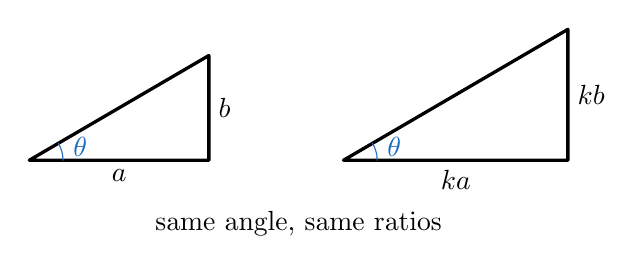
\begin{tikzpicture}[scale=0.95, line cap=round, line join=round]
  \definecolor{trigblue}{RGB}{30,110,190}
  \coordinate (A) at (0,0);
  \coordinate (B) at (2.4,0);
  \coordinate (C) at (2.4,1.4);
  \coordinate (D) at (4.2,0);
  \coordinate (E) at (7.2,0);
  \coordinate (F) at (7.2,1.75);
  \draw[very thick] (A)--(B)--(C)--cycle;
  \draw[very thick] (D)--(E)--(F)--cycle;
  \draw[trigblue] (0.45,0) arc[start angle=0,end angle=30.3,radius=0.45];
  \draw[trigblue] (4.65,0) arc[start angle=0,end angle=30.3,radius=0.45];
  \node[trigblue] at (0.68,0.18) {$\theta$};
  \node[trigblue] at (4.88,0.18) {$\theta$};
  \node[below] at (1.2,0) {$a$};
  \node[right] at (2.4,0.7) {$b$};
  \node[below] at (5.7,0) {$ka$};
  \node[right] at (7.2,0.88) {$kb$};
  \node[below] at (3.6,-0.55) {same angle, same ratios};
\end{tikzpicture}
\end{center}


\begin{theorembox}{Theorem}
\begin{theorem}[Well-definedness of sine and cosine]
\label{thm:sine-cosine-well-defined}
For each acute Euclidean angle $\theta$, the values $\sin\theta$ and
\(\cos\theta\) are independent of the right triangle chosen to compute them.
\end{theorem}
\end{theorembox}
\begin{remark*}[Standard quantified statement]
For every admissible input satisfying the hypotheses of the statement, the
displayed definition or assertion holds in the stated domain.
\end{remark*}

\begin{remark*}[Interpretation]
The statement records the named trigonometric object or identity together with
its intended domain of use.
\end{remark*}

\begin{remark*}[Proof]
\hyperref[prf:sine-cosine-well-defined]{Go to proof.}
\end{remark*}
\begin{dependencies}
\begin{itemize}
  \item \hyperref[def:acute-angle-sine]{Acute-angle sine}
  \item \hyperref[def:acute-angle-cosine]{Acute-angle cosine}
  \item \hyperref[thm:trig-ratios-similarity-invariant]{Similarity invariance of trigonometric ratios}
\end{itemize}
\end{dependencies}

\begin{center}
\begin{tikzpicture}[scale=1.05, line cap=round, line join=round]
  \definecolor{trigblue}{RGB}{30,110,190}
  \coordinate (A) at (0,0);
  \coordinate (B) at (3.2,0);
  \coordinate (C) at (3.2,1.85);
  \draw[very thick] (A)--(B)--(C)--cycle;
  \draw (2.9,0)--(2.9,0.3)--(3.2,0.3);
  \draw[trigblue] (0.5,0) arc[start angle=0,end angle=30,radius=0.5];
  \node[trigblue] at (0.72,0.2) {$\theta$};
  \node[below] at ($(A)!0.5!(B)$) {$a$};
  \node[right] at ($(B)!0.5!(C)$) {$o$};
  \node[above left] at ($(A)!0.5!(C)$) {$h$};
  \node[right] at (4.0,1.45) {$\sin=o/h,\quad \cos=a/h$};
  \node[right] at (4.0,0.95) {$\tan=o/a,\quad \cot=a/o$};
  \node[right] at (4.0,0.45) {$\sec=h/a,\quad \csc=h/o$};
\end{tikzpicture}
\end{center}


\begin{theorembox}{Theorem}
\begin{theorem}[Six trigonometric functions]
\label{thm:six-trig-functions}
The six right-triangle trigonometric ratios define functions of an acute
Euclidean angle, subject to the denominator restrictions in their defining
quotients.
\end{theorem}
\end{theorembox}
\begin{remark*}[Standard quantified statement]
For every admissible input satisfying the hypotheses of the statement, the
displayed definition or assertion holds in the stated domain.
\end{remark*}

\begin{remark*}[Interpretation]
The statement records the named trigonometric object or identity together with
its intended domain of use.
\end{remark*}

\begin{remark*}[Proof]
\hyperref[prf:six-trig-functions]{Go to proof.}
\end{remark*}
\begin{dependencies}
\begin{itemize}
  \item \hyperref[def:right-triangle-sine]{Right-triangle sine}
  \item \hyperref[def:right-triangle-cosine]{Right-triangle cosine}
  \item \hyperref[thm:sine-cosine-well-defined]{Well-definedness of sine and cosine}
\end{itemize}
\end{dependencies}

\begin{remark*}[Debt flag]
This definition extends sine and cosine beyond acute angles. Treating
$\theta$ as an arbitrary real-valued radian input requires arc length and
rectifiability machinery not yet developed in this volume.
\end{remark*}
\begin{dependencies}
\begin{itemize}
  \item \hyperref[def:euclid-circle]{Circle}
  \item \hyperref[def:cartesian-product]{Cartesian Product}
  \item \hyperref[thm:sine-cosine-well-defined]{Well-definedness of sine and cosine}
\end{itemize}
\end{dependencies}

\begin{center}
\begin{tikzpicture}[scale=1.45, line cap=round, line join=round]
  \definecolor{trigblue}{RGB}{30,110,190}
  \coordinate (O) at (0,0);
  \coordinate (P) at (32:1);
  \coordinate (Q) at ({cos(32)},0);
  \draw[gray!55] (O) circle (1);
  \draw[->] (-0.15,0)--(1.3,0) node[right] {$x$};
  \draw[->] (0,-0.15)--(0,1.15) node[above] {$y$};
  \draw[very thick] (O)--(Q)--(P)--cycle;
  \draw[trigblue] (0.3,0) arc[start angle=0,end angle=32,radius=0.3];
  \node[trigblue] at (0.35,0.1) {$\theta$};
  \node[below] at ($(O)!0.5!(Q)$) {$\cos\theta$};
  \node[right] at ($(Q)!0.5!(P)$) {$\sin\theta$};
  \node[above left] at ($(O)!0.5!(P)$) {$1$};
\end{tikzpicture}
\end{center}


\begin{theorembox}{Theorem}
\begin{theorem}[Unit-circle agreement with right-triangle trigonometry]
\label{thm:unit-circle-agrees-with-right-triangle-trig}
For $0<\theta<90^\circ$, the unit-circle definitions of sine and cosine agree
with the right-triangle definitions.
\end{theorem}
\end{theorembox}
\begin{remark*}[Standard quantified statement]
For every admissible input satisfying the hypotheses of the statement, the
displayed definition or assertion holds in the stated domain.
\end{remark*}

\begin{remark*}[Interpretation]
The statement records the named trigonometric object or identity together with
its intended domain of use.
\end{remark*}

\begin{remark*}[Proof]
\hyperref[prf:unit-circle-agrees-with-right-triangle-trig]{Go to proof.}
\end{remark*}
\begin{dependencies}
\begin{itemize}
  \item \hyperref[def:acute-angle-sine]{Acute-angle sine}
  \item \hyperref[def:acute-angle-cosine]{Acute-angle cosine}
  \item \hyperref[def:unit-circle-cosine]{Unit-circle cosine}
  \item \hyperref[def:unit-circle-sine]{Unit-circle sine}
\end{itemize}
\end{dependencies}

\begin{dependencies}
\begin{itemize}
  \item \hyperref[def:unit-circle-cosine]{Unit-circle cosine}
  \item \hyperref[def:unit-circle-sine]{Unit-circle sine}
  \item \hyperref[thm:unit-circle-agrees-with-right-triangle-trig]{Unit-circle agreement with right-triangle trigonometry}
\end{itemize}
\end{dependencies}

\begin{center}
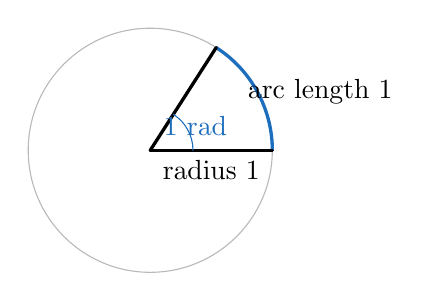
\begin{tikzpicture}[scale=1.55, line cap=round, line join=round]
  \definecolor{trigblue}{RGB}{30,110,190}
  \coordinate (O) at (0,0);
  \draw[gray!55] (O) circle (1);
  \draw[very thick,trigblue] (1,0) arc[start angle=0,end angle=57.3,radius=1];
  \draw[very thick] (O)--(1,0);
  \draw[very thick] (O)--(57.3:1);
  \draw[trigblue] (0.35,0) arc[start angle=0,end angle=57.3,radius=0.35];
  \node[trigblue] at (0.37,0.2) {$1$ rad};
  \node[right] at (0.72,0.48) {arc length $1$};
  \node[below] at (0.5,0) {radius $1$};
\end{tikzpicture}
\end{center}


\begin{definitionbox}{Definition}
\begin{definition}[Radian measure]
\label{def:radian-measure}
One radian is the angle that cuts off arc length $1$ on the unit circle. A full
turn has measure $2\pi$ radians.
\end{definition}
\end{definitionbox}
\begin{remark*}[Standard quantified statement]
For every admissible input satisfying the hypotheses of the statement, the
displayed definition or assertion holds in the stated domain.
\end{remark*}

\begin{remark*}[Interpretation]
The statement records the named trigonometric object or identity together with
its intended domain of use.
\end{remark*}

\begin{remark*}[Debt flag]
This definition uses arc length intuitively. Its rigorous foundation belongs
after rectifiable curves and the construction of $\pi$ from circumference.
\end{remark*}
\begin{dependencies}
\begin{itemize}
  \item \hyperref[def:unit-circle-cosine]{Unit-circle cosine}
  \item \hyperref[def:unit-circle-sine]{Unit-circle sine}
  \item \hyperref[def:euclid-circle]{Circle}
\end{itemize}
\end{dependencies}
